\section{Discussion}

\subsection{Fault Injection}

To analyze the difference in fault tolerance between fixed and floating point numbers, there are some assumptions that need to be made. 

This comparison is based on injecting faults within the data that is being operated on, not on instruction bits or any other part of the program. The fault locations are selected based on operations that are only done a few of in the program, such as division, to be able to inject a fault in an equivalent location for all the different versions of the program. The comparison does not hold for anything other than an injection of faults in the data. 

Fixed point and floating point representations require different hardware to execute, or at least emulation of the missing instructions. this leads to significantly different code, using different parts of the processor. Were a bit to be flipped in the same memory location when both programs are running, there is a high likelihood of the bit being flipped representing very different parts in the respective programs. 




The results of the fault injection campaign completed for the seidel-2d benchmark from the polybench cpu benchmark suite adapted for \taffo is not representative for programs compiled with \taffo as a whole. The changes that are made to the low-level code vary from project to project depending on the domain, and depends on what the user of the program specifies to be the range of values. 

The results from the fault injection were mostly expected: The deviations from the original answer for the floating point errors started low, then skyrocketed exponentially towards the most significant bits.




% explanation of floating point implementation
% explanation of fixed point implementatoin
% diagrams

% The LLVM-IR documentation states that when shifting the value beyond the bounds of number being shifted, you should get undefined behavior~\cite{LLVM_language_reference}. This can be seen in the experiment when attempting to inject faults in bits that don't exist. When injecting bits beyond the 64 that exist in the variable, the results become unpredictable for the fixed point implementations, and invalid for the floating point value. This however is not relevant to this thesis but concerns llvm IR behavior, and will therefore be ignored.

In the output file of the original floating point implementation without any additional faults injected, there are 17 significant digits, 16 of which is behind the decimal point. An error above 1 could therefore be considered to be quite a large error. Figure~\ref{fig:graph_fixed_vs_float_error} shows a graph of how the  deviations in the output change when flipping a single bit in equivalent locations for a floating point and fixed point implementation. The deviation is the accumulated average absolute difference for each data point compared to the original floating point implementation of the program without additional faults injected. The x axis describes which bit is flipped, bit number 0 being the least significant bit.

\begin{figure}[h!]
    \centering
    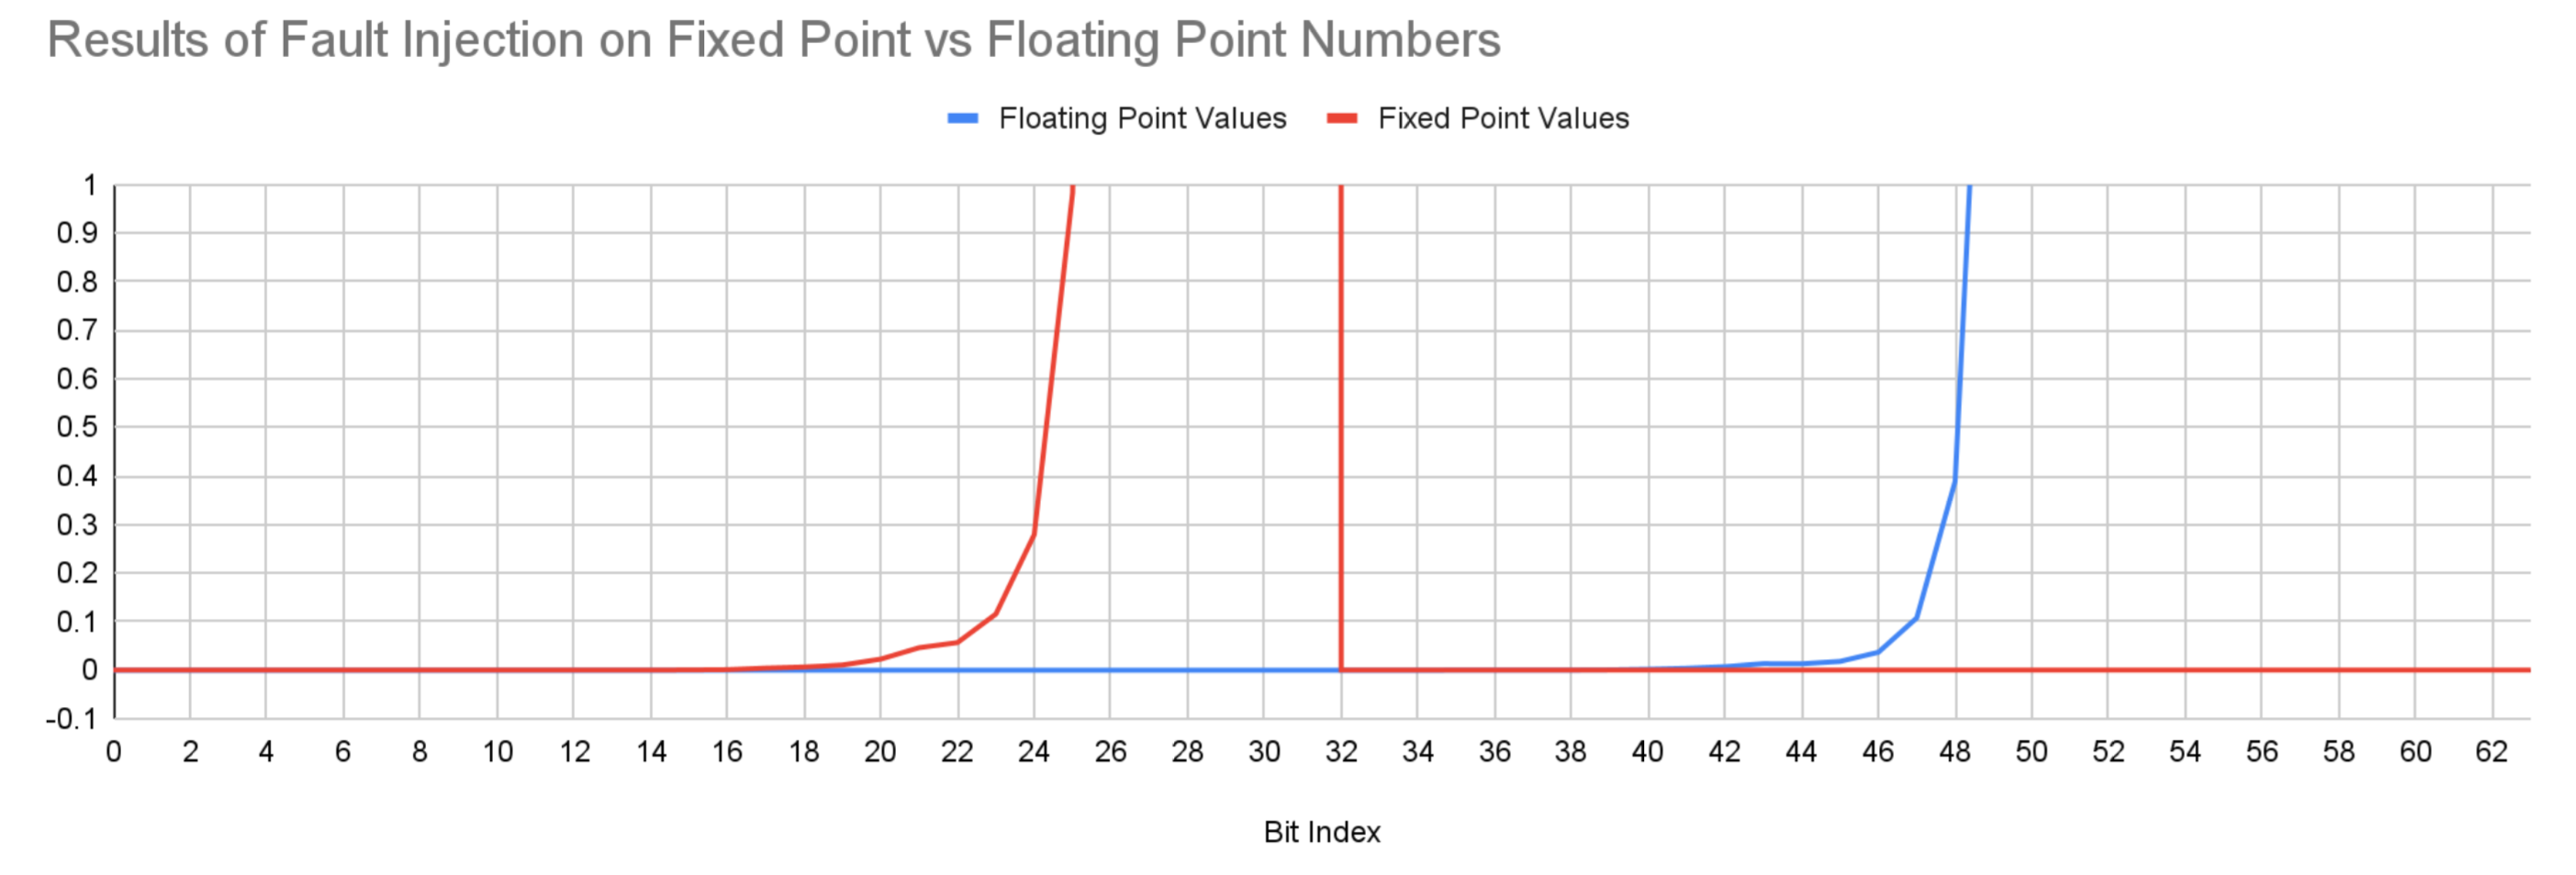
\includegraphics[width=0.5\linewidth]{Images/graph_float_vs_fixed_fault_injection_results.png}
    \caption{The graph shows how the difference from the original floating point version of the program increases the closer to the most significant bit the fault is injected. }
    \label{fig:graph_fixed_vs_float_error}
\end{figure}


The graph y axis starts at negative values even though this is not possible (the y axis is average absolute difference, negative or positive doesn't matter) to more clearly show the line for the floating point data, as they are very close to being zero.

The graph shows that both the floating point values and the fixed point values seem to differ very little from the original non-fault-injected outputs. The difference in the fixed point implementation rises quickly as the injected bit approaches the the most significant bit, until suddenly dropping after injection in the bit at index 32. This can be explained by looking at the LLVM-IR that is used to inject the faults. 

% FIGURE: LLVM IR OF FIXED POINT

\begin{figure}[h!]
    \centering
    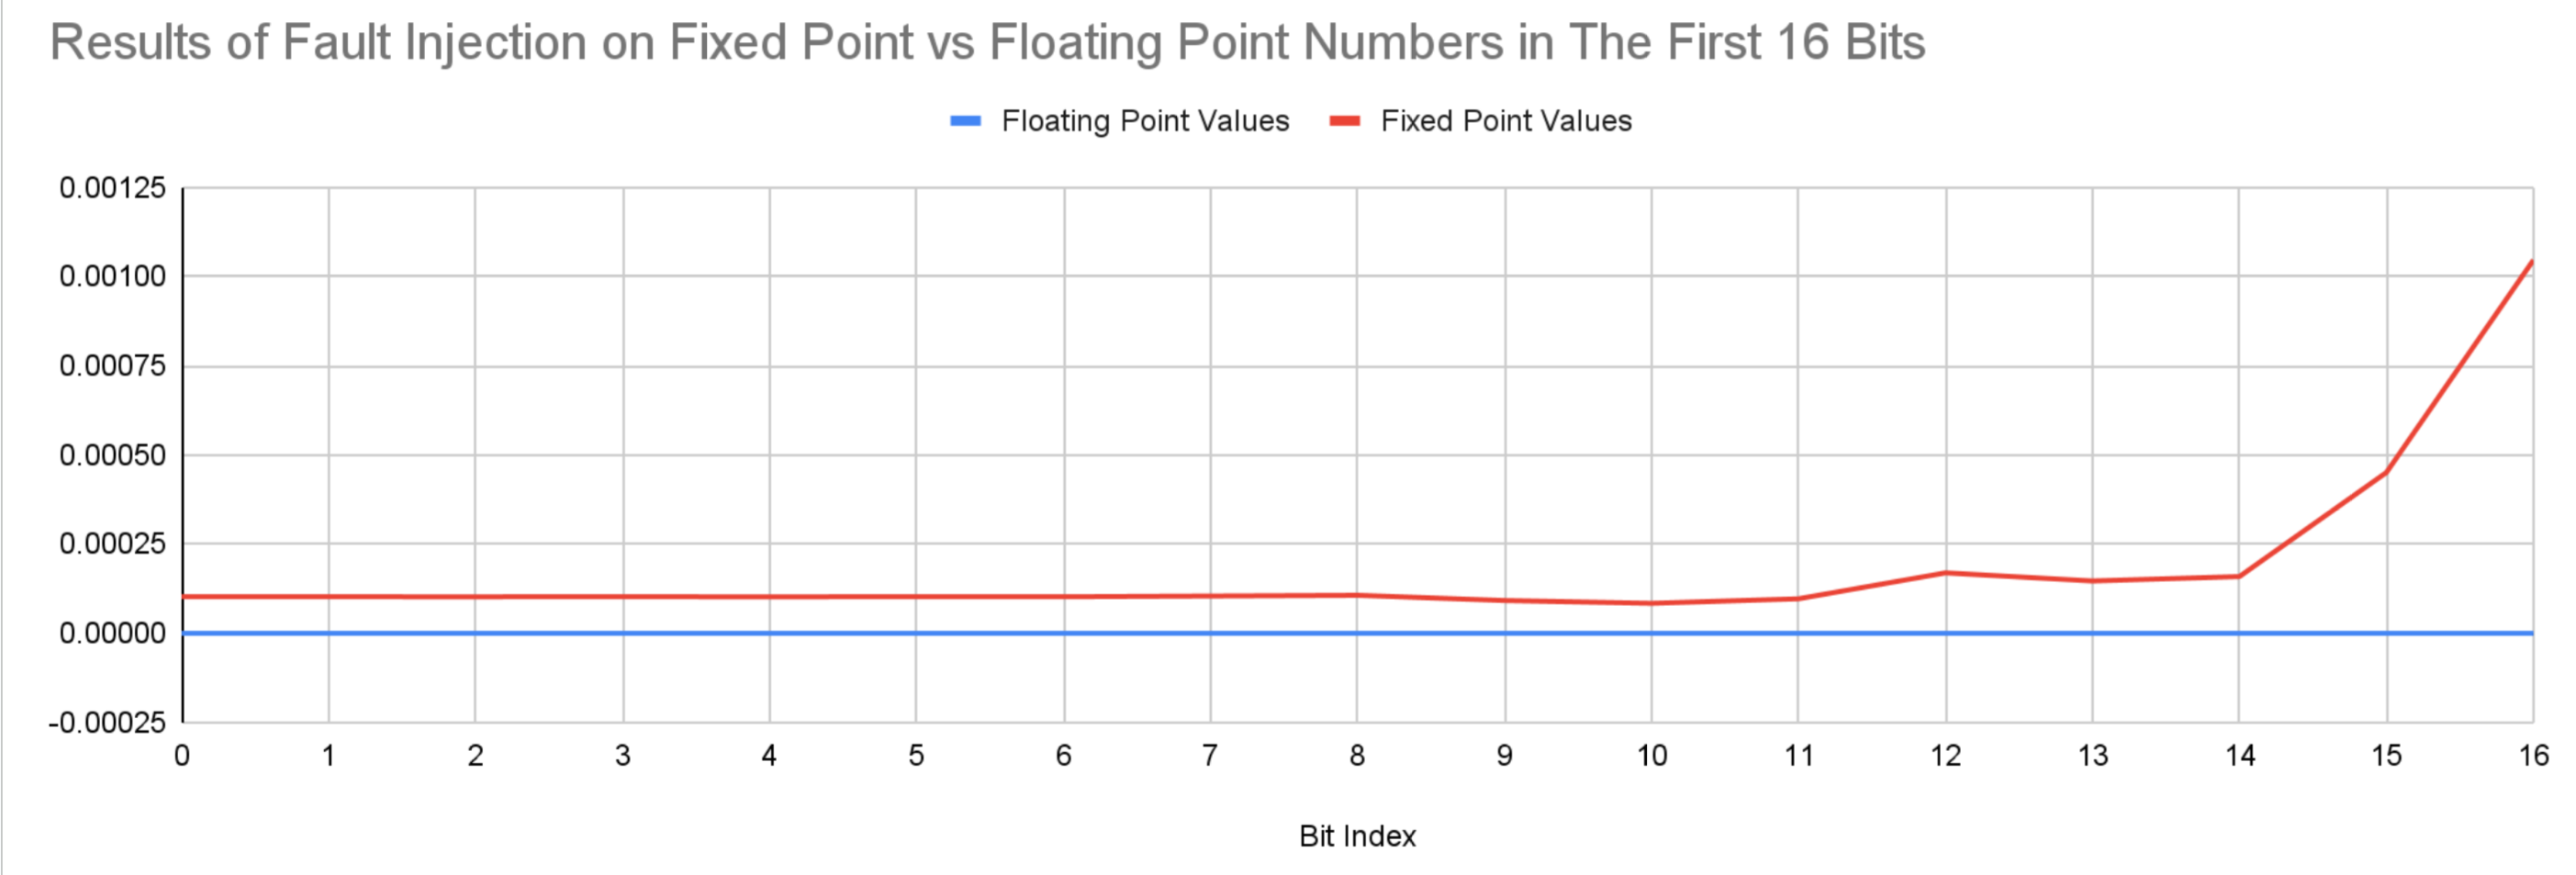
\includegraphics[width=0.5\linewidth]{graph_fault_injection_fix_vs_float_first_16_bits.png}
    \caption{The fixed point error is magnitudes larger than the floating point error at its lowest.}
    \label{fig:graph_fixed_vs_float_error_first_16}
\end{figure}

When assessing how the injected faults affect the behavior of the tools, it is helpful to use the failure classifications found in~\citet{failure_class_with_respect_to_detection} for subtle incorrect-- and coarse incorrect service values. A service is the behavior of a system as percieved by an external observer. For a perfect observer, i.e. an observer that can accurately map a service output as either a correct or incorrect output. Humans are rarely perfect, which puts us in a different category able to discern between three different states of service delivery: correct, coarse incorrect, and subtle incorrect.  Coarse incorrect are states that are certainly false, correct states are observably correct, and subtle incorrect states are difficult to discern as being incorrect or correct. This means that a value could be percieved as correct while actually being the result of faulty service, i.e. an error (according to laprie).

This is why the domain matters when discussing reliability. In the result, until injecting a fault in bit number 37 from the right, the floating point error remains lower than that of the fixed point implementation with no faults injected. At bit number 55 from the left, the error becomes larger than the highest error recorded for the fixed point implementations, and the error keeps rising until injecting an error at bit number 64 from the left, which is the sign bit.

If we define the standard fixed point version as the threshold for a coarse error, the majority of bit flips do not constitute a fault, but keeps it within the range of what could be a successful service delivery. 


For this concrete benchmark, the precision was set such as to allow the use of 32 bit integers for the fixed point implementation. This explains why above bit 32 from the right, the error goes back to the same error as the fault free fixed point implementation. This may not be the case for all workloads. 



% discuss the error, how error rate changes with injected bit, implications taking subtle and coarse errors into account. Subtle errors may have a larger effect on scientific calculations or highly sensitive calculations such as for satellite navigation or space travel, where if travelling very long distances a small error may result in a huge deviation. Larger errors may be easier to discover.
A larger deviation may be easier to discover than a lower deviation. Either through statistics or other detection algorithms. The fact that many bits in a 64-bit floating point number can be injected without a significant effect on the calculation may be an advantage if the calculation in question is fault tolerant at heart. Floating point errors go up very quickly when the error hits the exponent part of the number, so detecting a fault above a certain threshold is feasible.

On the other hand, while the smallest faults injected into fixed point numbers are larger than the smallest faults in floating point numbers, a number where only the 32 lowest bits will affect the calculations that follow have 32 bits where nothing happens when they are flipped. This is taking the huge assumption that only data bits are flipped, when this is not necessarily the case at all.




\subsection{code changes}

On a different note, the code changes of the validation script result in a more understandable piece of software.

The comparison script written for the fault injection comparison is not perfect either. However, the assumptions are documented, and tests support and explain functionality. This is difficult to realize when using python as a scripting language, but at the very least variable names need to be descriptive, and file outputs need to follow the existing standards and descriptions (for instance not mislabeling an output as a .csv file).

Some changes were apparent not because of the programming skills of the author, but simply because of an IDE tool highlighting errors that were easy to remedy. There is a habit of writing code as if to be archived forever. The documentation lags behind, and there is no test suite for the tool
